\documentclass[10pt,unknownkeysallowed]{beamer}
\usepackage{beamerthemesplit} % new 
\usepackage{media9}
\usepackage{multimedia}
\usepackage{tcolorbox}
\usepackage{hyperref}
\usepackage{tikz}
\usepackage{pgfplots}
\usepackage{graphicx}

\usetheme{Frankfurt}
%\usetheme{Madrid}
%\usetheme{Copenhagen}

%Document begins
\begin{document}
\title{\textcolor{green}{M}usic, \textcolor{green}{M}achine, and \textcolor{green}{M}athematics} 
\author{\textbf{\textcolor{green}{M}annan, \textcolor{green}{M}ajhi}}
%\date{\today} 
\date{\textcolor{green}{M}arch 24, 2015}
\frame{\titlepage} 

\frame{\frametitle{Overview}\tableofcontents} 

\section{Introduction To Music} 
\begin{frame}{Mysterious Melody(Diana Deutsch, 1972)}
  \begin{tcolorbox}[colback=green!5,colframe=green!40!black,title=Scrambled]
    \movie[inline, samplingrate=44100,bitspersample=16,showcontrols=true]{\textcolor{red}{ClickToPlay}}{1.mp3}\\
  \end{tcolorbox}
  \pause
  \begin{tcolorbox}[colback=green!5,colframe=green!40!black,title=UnScrambled]
    \movie[inline, samplingrate=44100,bitspersample=16,showcontrols=true]{\textcolor{green}{ClickToPlay}}{2.mp3}\\
  \end{tcolorbox}
  \pause
  \begin{tcolorbox}[colback=green!5,colframe=green!40!black,title=Conclusion]
    \textcolor{blue}{Sound(Physics) + Ear(Biology) + Brain(??) = Perception Of Sound(What We Hear)!}
  \end{tcolorbox}
\end{frame}

\frame{\frametitle{Physics Of Sound} 
  \begin{block}{Sound}
    \textbf{Sound} is created by repetitive pressure change in the air. We can hear it when the repetition occurs roughly 20 
    to 20000 times a second.
  \end{block}
  \begin{block}{Components Of Sound}
    A \textbf{Musician} describes a sustained, musical tone in terms of three quantities:\\
    \begin{itemize}
    \item \textbf{Pitch}
    \item \textbf{Loudness}
    \item \textbf{Timbre}
    \end{itemize}
    A \textbf{Physicist} would describe the same tone in terms of three quantities:\\
    \begin{itemize}
    \item \textbf{Frequency}
    \item \textbf{Intensity}
    \item \textbf{Overtone or Harmonic Structure}
    \end{itemize}
  \end{block}
}

\frame{\frametitle{Sound From A Piano}
      \begin{figure}
        \centering
        \includegraphics[scale=0.7]{piano.jpg}
        \caption{Piano (A below C4)}
      \end{figure}
      
  %\movie[inline, samplingrate=44100,bitspersample=16,showcontrols=true]{\textcolor{red}{ClickToPlay}}{three_sounds.mp3}\\
  \textcolor{red}{\href{http://www.phy.mtu.edu/~suits/notefreqs.html}{Frequency Chart}}
}

\frame{\frametitle{Pitch/Frequency}  
  \begin{block}{Observation}
    Musical tones are generated by (almost) periodic change of pressure in the air. The period(frequency) is perceived as 
    the \textbf{Pitch} of the tone. 
  \end{block}
  
  \begin{block}{11000 To 20000 Hertz}
    How many you could hear? How old are you?
    \movie[inline, samplingrate=44100,bitspersample=16,showcontrols=true]{\textcolor{red}{ClickToPlay}}{11to20khz.mp3}\\
  \end{block}
  \begin{block}{Perception Of Frequency Is \textcolor{green}{Not Linear}}
    This plays tones of pitch evenly spaced: 500,1500, 2500, 3500, 4500, 6500 Hertz.
    \movie[inline, samplingrate=44100,bitspersample=16,showcontrols=true]{\textcolor{red}{ClickToPlay}}{even_freq.mp3}\\
  \pause You will perceive them to be getting closer together in frequency instead. So even spacing in frequency is not the 
    natural perception of even spacing in pitch. 
  \end{block}
  \pause
  \begin{block}{Perception Of Frequency Is \textcolor{green}{Logarithmic(Base 2)}}
    Do these sound evenly spaced?
    \movie[inline, samplingrate=44100,bitspersample=16,showcontrols=true]{\textcolor{red}{Ratio2}}{octaves.mp3}
    %\movie[inline, samplingrate=44100,bitspersample=16,showcontrols=true]{\textcolor{red}{Ratio3/2}}{fifths.mp3}\\
  \end{block}
}

\frame{\frametitle{Loudness/Intensity} 
  \begin{block}{Definition}
    \begin{itemize}
    \item To a physicist ``Intensity$=$\textbf{Power/Area}''. 
    \item To a musician ``how loud it sounds to his ear''(\textbf{which depends on one's perception}).
    \end{itemize} 
  \end{block}
  
  \begin{block}{Range Of Perceivable Loundness}
    Just as we hear sounds which occur in a wide range of frequencies, we hear sounds in a very wide range of loudnesses. 
    Sometimes it is important to be able to hear that someone is breathing in the same room as you. Sometimes someone will 
    shout in your ear. The sound intensity of the shout may be more than a billion times larger than the loudness of the 
    breathing. You have to be able to usefully perceive both.
  \end{block}
}

\frame{\frametitle{Loundness/Intensity}
  \begin{block}{}
    Perception of loudness is \textcolor{green}{Not Linear} again!
    \textbf{The actual relation of intensity with loudness has to do with how the neurons are 
      triggered by the intensity and duration of sound}.
  \end{block}
  \begin{block}{Measuring Loudness}
    A standard way to measure loudness is \textbf{Bel} which is be definition\\
    $1 Bel=log_{10}\frac{Intensity}{10^{-12} W/m^2}$\\
    1 Bel is too loud!
    For practical purposes we use \textbf{deciBel = $\frac{1}{10}$ Bel}. 
  \end{block} 
  \begin{block}{A Rule Of Thumb}
    \textbf{10 TIMES INCREASE IN INTENSITY IS PERCEIVED AS A 2 TIMES INCREASE IN PERCEIVED LOUDNESS}.
    \movie[inline, samplingrate=44100,bitspersample=16,showcontrols=true]{\textcolor{red}{ClickToPlay}}{loud_soft.mp3}\\
  \end{block}
}

\frame{\frametitle{Pitch And Loudness Are Not Independent}
  \begin{block}{}
    Tones of the same intensity, but of different frequency, perceived as being of different loundness.\\
  \end{block}
  
  \begin{columns}[T]
    \begin{column}{0.9\textwidth}
      \begin{figure}
        \centering
        \includegraphics[scale=0.8,width = 0.5\textwidth]{ISO226.png}
        \caption{Equal Loudness Contours}
      \end{figure}
    \end{column}
    \begin{column}{0.5\textwidth}
      \textcolor{red}{\href{http://newt.phys.unsw.edu.au/jw/hearing.html}{HearingTestWebsite}}
    \end{column}
  \end{columns}
}
\section{Storing And Reproducing Sound}
\begin{frame}
\frametitle{Computer Generation of Sound}
\begin{block}{What is Sound on a computer?}

\begin{tikzpicture}[domain =0:6.14, scale = 0.5]
\draw[thick,color=black, ->] (0,0)-- (6.14,0);
\draw[thick, color=black, <->] (0,-1) -- (0,1);
\draw [red] plot  (\x,{sin(\x r)});

\draw[thick,color=black, ->] (14,0)-- (14+6.14,0);
\draw[thick, color=black, <->] (14,-1) -- (14,1);
%\filldraw circle (6,0) (2 pt);
\foreach \i in {1,...,7}{
\pgfmathsetmacro{\y}{sin((\i-1) r)}

\filldraw[red] (14+\i-1,\y) circle (2 pt);

}
\node[draw, rectangle, anchor = west] at (10,0) {$\Large \rightarrow$};
\end{tikzpicture}


\end{block}


\begin{block}{Then to a speaker}
\begin{tikzpicture}[domain =0:6.14, scale = 0.5]
\draw[thick,color=black, ->] (0,0)-- (6.14,0);
\draw[thick, color=black, <->] (0,-1) -- (0,1);
\foreach \i in {1,...,7}{
\pgfmathsetmacro{\y}{sin((\i-1) r)}

\filldraw[red] (\i-1,\y) circle (2 pt);

}
\node[draw, rectangle, anchor = west] at (10,0) {$\Large \rightarrow$};
\node[anchor = west] at (14,0) {\includegraphics[width = 0.25\textwidth]{speaker.png}};
\end{tikzpicture}


\end{block}
\end{frame}


\begin{frame}
\frametitle{How to choose the sampling rate}
\begin{block}{Sampling rate = discretization}
That is to say, the sampling rate has the same issues as discretization choices do in numerical mathematics. How can the necessary information be captured most efficiently?
\end{block}

\begin{block}{CDs}
CDs use 44.1 kHz sampling. Why?
\end{block}
\end{frame}

\begin{frame}
\frametitle{Capturing a pressure wave}
\begin{block}{Sampling at 1.75 of the period}
\begin{tikzpicture}[domain =0:50, scale = 0.25, samples = 100]
\draw [red] plot  (\x,{sin(\x r)});
\foreach \i in {1,...,6}{
\pgfmathsetmacro{\x}{3.14*2*(1.75)*(\i-1)}
\pgfmathsetmacro{\y}{sin(\x r)}
\filldraw[black] (\x,\y) circle (3 pt);
}
\end{tikzpicture}
\end{block}

\begin{block}{Sampling at 0.75 of the period}
\begin{tikzpicture}[domain =0:50, scale = 0.25, samples = 100]
\draw [red] plot  (\x,{sin(\x r)});
\foreach \i in {1,...,10}{
\pgfmathsetmacro{\x}{3.14*2*(0.75)*(\i-1)}
\pgfmathsetmacro{\y}{sin(\x r)}
\filldraw[black] (\x,\y) circle (2 pt);
}
\end{tikzpicture}
\end{block}

\begin{block}{Sampling at 0.45 of the period}
\begin{tikzpicture}[domain =0:50, scale = 0.25, samples = 100]
\draw [red] plot  (\x,{sin(\x r)});
\foreach \i in {1,...,25}{
\pgfmathsetmacro{\x}{3.14*2*(0.45)*(\i-1)}
\pgfmathsetmacro{\y}{sin(\x r)}
\filldraw[black] (\x,\y) circle (2 pt);
}
\end{tikzpicture}
\end{block}
\end{frame}

\begin{frame}
\frametitle{Nyquist}

\begin{block}{Nyquist-Shannon Theorem}
If a function $Q$ is composed of continuous periodic waves (i.e. a nice fourier series) and has a highest frequency component in hertz  $f_{max}$ then the data of a sampling rate of at least $2f_{max}$ can be used to exactly determine $Q$.
\end{block}

\end{frame}


\section{Music With Machine}
\begin{frame}
 Pd Examples
 \end{frame}
 

\begin{frame}
\frametitle{How Can 2 Sound Waves Interact?}
\begin{block}{First, what happens when two sound waves meet?}
They add.
\end{block}

\end{frame}

\begin{frame}
\frametitle{The math of 2 wave friends}
\begin{block}{Wave$_1$ \& Wave$_2$}
Suppose Wave$_1 = A\cos(wt + k)$ and Wave$_2 = A\cos(w't + k')$. Then,
\begin{align*}
W_1 + W_2 =&A\cos(wt + k) + A\cos(w't + k')\\
=&2A\cos(\frac{(w+w')t+(k+k')}{2})\cos(\frac{(w-w')t +(k- k')}{2})
\end{align*}
\end{block}

\end{frame}

\begin{frame}
\frametitle{Aural Beating}
\begin{block}{The math of the given example}
Suppose Wave$_1 = \cos(440t)$ and Wave$_2 = \cos(435t)$. Then,
\begin{align*}
W_1 + W_2 =&\cos(440t) + \cos(435t)\\
=&2\cos(\frac{875t}{2})\cos(\frac{5t}{2})
\end{align*}
\end{block}

\begin{block}{}
\center 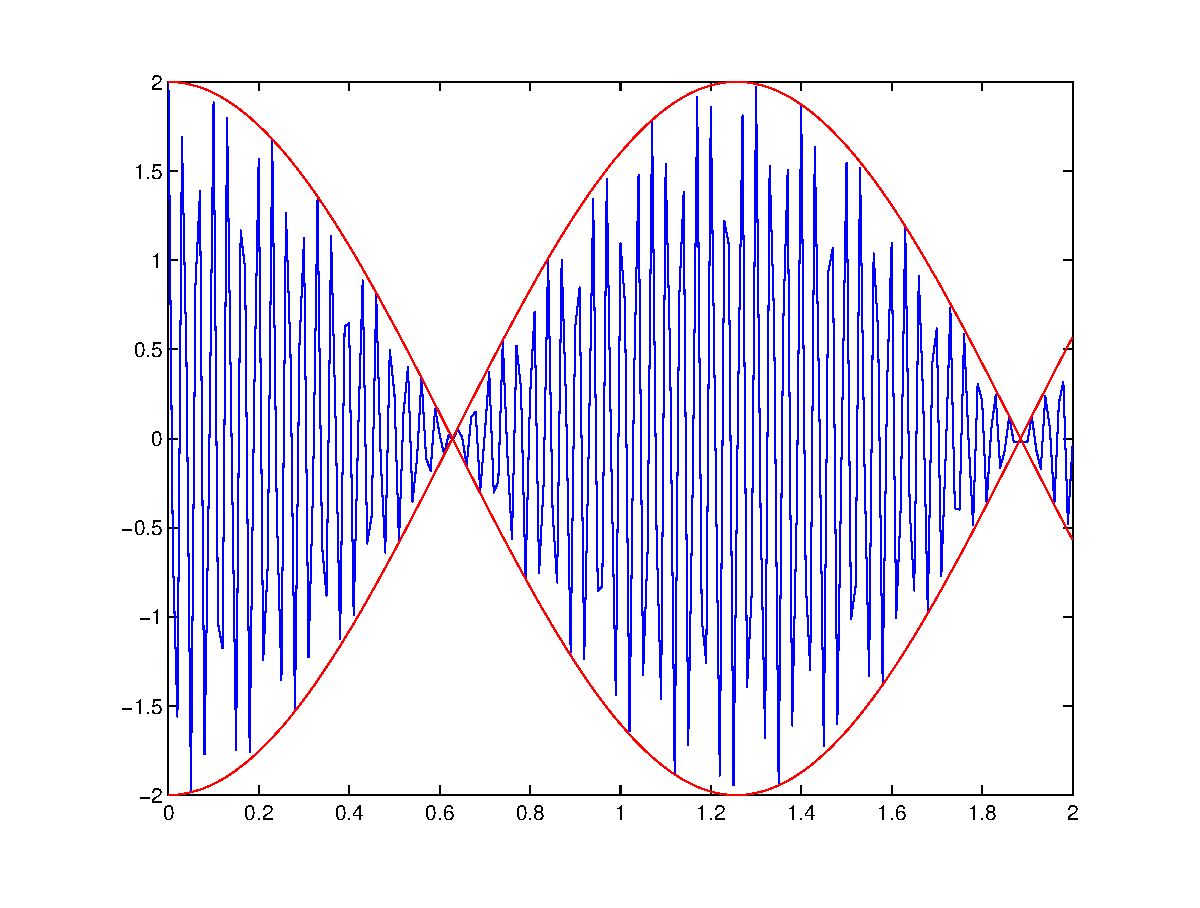
\includegraphics[width = 0.5\textwidth]{BeatingWave.eps}
\end{block}


\end{frame}

\begin{frame}
\frametitle{Computer Generation of Sound}
\begin{block}{What is Sound on a computer?}

\begin{tikzpicture}[domain =0:6.14, scale = 0.5]
\draw[thick,color=black, ->] (0,0)-- (6.14,0);
\draw[thick, color=black, <->] (0,-1) -- (0,1);
\draw [red] plot  (\x,{sin(\x r)});

\draw[thick,color=black, ->] (14,0)-- (14+6.14,0);
\draw[thick, color=black, <->] (14,-1) -- (14,1);
%\filldraw circle (6,0) (2 pt);
\foreach \i in {1,...,7}{
\pgfmathsetmacro{\y}{sin((\i-1) r)}

\filldraw[red] (14+\i-1,\y) circle (2 pt);

}
\node[draw, rectangle, anchor = west] at (10,0) {$\Large \rightarrow$};
\end{tikzpicture}


\end{block}


\begin{block}{Then to a speaker}
\begin{tikzpicture}[domain =0:6.14, scale = 0.5]
\draw[thick,color=black, ->] (0,0)-- (6.14,0);
\draw[thick, color=black, <->] (0,-1) -- (0,1);
\foreach \i in {1,...,7}{
\pgfmathsetmacro{\y}{sin((\i-1) r)}

\filldraw[red] (\i-1,\y) circle (2 pt);

}
\node[draw, rectangle, anchor = west] at (10,0) {$\Large \rightarrow$};
\node[anchor = west] at (14,0) {\includegraphics[width = 0.25\textwidth]{speaker.png}};
\end{tikzpicture}


\end{block}
\end{frame}

\begin{frame}
\begin{block}{Sampling at $\Delta t$}
\begin{tikzpicture}[domain =0:30, scale = 0.4, samples = 100]
\draw[thick,color=black, ->] (0,0)-- (6.14,0);
\draw [red] plot  (\x,{sin(\x r)});
\foreach \i in {1,...,7}{
\pgfmathsetmacro{\x}{ 0.78*(\i-1)+0.78*(\i-1)}
\pgfmathsetmacro{\y}{sin( \x r)}

\filldraw[red] (\x,\y) circle (2.5 pt);

}

\end{tikzpicture}

%\begin{tikzpicture}[domain =0:6.14, scale = 0.5]
%\draw[thick,color=black, ->] (0,0)-- (6.14,0);
%\draw [red] plot  (\x,{sin(\x r)});
%\foreach \i in {1,...,7}{
%\pgfmathsetmacro{\y}{sin((\i-1) r)}
%
%\filldraw[red] (\i-1,\y) circle (2 pt);
%
%}
%\end{tikzpicture}
\end{block}

\begin{block}{Sampling at same rate of a higher frequency tone}
\begin{tikzpicture}[domain =0:30, scale = 0.4, samples = 500]
\draw[thick,color=black, ->] (0,0)-- (6.14,0);
\draw [red] plot  (\x,{sin(5*\x r)});
\foreach \i in {1,...,7}{
\pgfmathsetmacro{\x}{  0.78*(\i-1)+0.78*(\i-1)}
\pgfmathsetmacro{\y}{sin( \x r)}

\filldraw[red] (\x,\y) circle (2.5 pt);

}

\end{tikzpicture}
\end{block}


\end{frame}

\section{Pure SineWaves Are Not Natural}

\begin{frame}
\frametitle{Sounds from instruments}

\begin{block}{Fundamental and overtones}
\center \includegraphics[scale = 0.75]{Harmonics.png};
\end{block}

\end{frame}


\frame{\frametitle{How We Hear} 
  \begin{tikzpicture}
    \draw[color=blue][style=thick] (0,0) rectangle (4,1);
    \foreach \x in {80,...,0}
    \draw[color=blue][-] (0+4*\x/80,1) -- (0+4*\x/80,0);
    \tikzstyle{every node} = [circle, fill=gray!30]
    \node (a) at (2,0.5) {Ear};
    \node (b) at (2,3) {Input:Periodic f};
    \node (c) at (8,0.5){Output:(Pitch,Loudness)};
    \draw[color=blue][->] (b) -- (2,1);
    \draw[color=blue][->] (4,0.5) -- (c);
    \draw[line width=1pt][color=red] (3,0) to [out=105, in=-50] (3,1);
  \end{tikzpicture}
  %% \begin{block}{Bad News}
  %%   \textcolor{red}{We can only hear simple Sine tones!}
  %% \end{block}
}

\frame{\frametitle{Some Random Sounds}
  \begin{columns}[T]
    \begin{column}{0.6\textwidth}
      \begin{figure}
        \centering
        \includegraphics[scale=0.7,width = 0.45\textwidth]{wineglass.jpg}
        \caption{Wineglass}
      \end{figure}
      \begin{figure}
        \centering
        \includegraphics[scale=0.7,width = 0.45\textwidth]{whistle.jpg}
        \caption{Whistle}
      \end{figure}
    \end{column}
    \begin{column}{0.6\textwidth}
      \begin{figure}
        \centering
        \includegraphics[scale=0.7,width = 0.45\textwidth]{siren.jpg}
        \caption{Siren}
      \end{figure}
      \begin{figure}
        \centering
        \includegraphics[scale=0.7,width = 0.45\textwidth]{voice.jpg}
        \caption{Voice}
      \end{figure}
    \end{column}
  \end{columns}
  \movie[inline, samplingrate=44100,bitspersample=16,showcontrols=true]{\textcolor{red}{ClickToPlay}}{three_sounds.mp3}\\
}

\frame{\frametitle{Fourier Analysis Of Sound}
  \begin{block}{Good News}
    \textcolor{green}{Superposition of sound works for our brain, the way superposition of waves works in nature!}\\
     If several things are producing sounds at once, then the pressure of the air, due to 
    the several things, will be\\
    $P_{air}=P_{atmospheirc}+P_{source 1}+P_{source 2}+...$
  \end{block}
  \begin{block}{Power Of Mathematics}
    As we have seen Our ears like periodic tones. And \textbf{Fourier} says, \textcolor{blue}{any periodic function $f(x)$, say the 
      pressure pattern from an instrument, can be viewed as the sum of many Sine waves}.   
  \end{block}
}


\frame{\frametitle{Timbre(Fourier Modes)}
  \begin{columns}[T]
    \begin{column}{0.6\textwidth}
      \begin{figure}
        \centering
        \includegraphics[scale=0.7,width = 0.65\textwidth]{Oboe.jpg}
        \caption{Oboe}
      \end{figure}
      \begin{figure}
        \centering
        \includegraphics[scale=0.7,width = 0.65\textwidth]{Piano1.jpg}
        \caption{Piano}
      \end{figure}
    \end{column}
    \begin{column}{0.6\textwidth}
      \begin{figure}
        \centering
        \includegraphics[scale=0.7,width = 0.65\textwidth]{Clarinet.jpg}
        \caption{Clarinet}
      \end{figure}
      \begin{figure}
        \centering
        \includegraphics[scale=0.7,width = 0.65\textwidth]{Flute.jpg}
        \caption{Flute}
      \end{figure}
    \end{column}
  \end{columns}
}

\frame{\frametitle{How To Produce Realistic Sounds}
  WaveForm Patch\\
  Synthesizer Patch\\
}

\frame{\frametitle{FM Synthesis}
 FM Synthethis Patch
}

\begin{frame}[plain,c]
%\frametitle{A first slide}

\begin{center}
\Huge Thank You!
\end{center}

\end{frame}


\end{document}
